\subsection{Slučaj upotrebe: Montaža filma}

\subsubsection*{Kratak opis}

Montažer iz odobrenih materijala (animiranih scena i zvuka) sastavlja montažu filma, određuje redosled i trajanje scena i dodaje zvuk. Završena montaža šalje se projektnom menadžeru na pregled.

\subsubsection*{Akteri}
\begin{itemize}
    \item \textbf{Montažer} -- sastavlja montažu filma, uređuje je i šalje na pregled.
    \item \textbf{Projektni menadžer} -- prima obaveštenje o montaži poslatoj na pregled.
\end{itemize}

\subsubsection*{Preduslovi}
\begin{itemize}
    \item Montažer je prijavljen na sistem i angažovan na projektu.
    \item Projekat animiranog filma postoji u sistemu i ima odobrene materijale.
\end{itemize}

\subsubsection*{Postuslovi}
\begin{itemize}
    \item Montaža je sačuvana u sistemu sa redosledom stavki, trajanjima i zvukom, a svaka izmena je zabeležena sa autorom i datumom.
    \item Ako je montaža poslata na pregled, projektni menadžer je obavešten.
\end{itemize}

\subsubsection*{Osnovni tok}
\begin{enumerate}
    \item Montažer bira projekat i opciju ,,Montaža filma''.
    \item Sistem prikazuje odobrene materijale projekta i trenutnu montažu.
    \item Montažer bira opciju ,,Dodaj stavku'' i unosi podatke o stavci montaže.
    \item Sistem proverava podatke, dodaje stavku u montažu i ažurira ukupno trajanje filma. Koraci 3 i 4 se ponavljaju dok montažer ne unese sve stavke.
    \item Po potrebi, montažer uređuje montažu: dodavanje zvuka stavci (podtok P1), promena redosleda i trajanja stavki (podtok P2) ili uklanjanje stavke iz montaže (podtok P3).
    \item Montažer bira opciju ,,Pošalji na pregled''.
    \item Sistem proverava da su sve scene uključene u montažu, menja status montaže u ,,Poslata na pregled'', obaveštava projektnog menadžera i prikazuje poruku o uspešnom slanju.
\end{enumerate}

\subsubsection*{Podtokovi}

\paragraph*{P1: Dodavanje zvuka stavci}
\begin{enumerate}
    \item Montažer bira stavku i opciju ,,Dodaj zvuk''.
    \item Montažer bira zvučni zapis i unosi podatke o zvuku.
    \item Sistem proverava podatke i povezuje zvuk sa stavkom.
\end{enumerate}
Podtok se poziva iz koraka 5 osnovnog toka, a po završetku se nastavlja od koraka 5.

\paragraph*{P2: Promena redosleda i trajanja stavki}
\begin{enumerate}
    \item Montažer bira stavku i unosi novi redni broj, odnosno novi početak i kraj isečka.
    \item Sistem proverava podatke, ažurira redosled i ukupno trajanje filma.
\end{enumerate}
Podtok se poziva iz koraka 5 osnovnog toka, a po završetku se nastavlja od koraka 5.

\paragraph*{P3: Uklanjanje stavke iz montaže}
\begin{enumerate}
    \item Montažer bira stavku i opciju ,,Ukloni iz montaže''.
    \item Sistem traži potvrdu, a montažer potvrđuje.
    \item Sistem uklanja stavku iz montaže i ažurira redosled i ukupno trajanje filma. Originalni materijal ostaje nepromenjen.
\end{enumerate}
Podtok se poziva iz koraka 5 osnovnog toka, a po završetku se nastavlja od koraka 5.

\subsubsection*{Alternativni tokovi}

\paragraph*{A1: Nepopunjena ili neispravna polja}
\begin{itemize}
    \item \textbf{Izaziva ga:} korak 4 osnovnog toka, kao i korak 3 podtoka P1 i korak 2 podtoka P2, ako neko obavezno polje nije popunjeno ili je neispravno (kraj isečka pre početka, isečak duži od materijala).
    \item \textbf{Ispravka:}
    \begin{enumerate}
        \item Sistem označava neispravna polja i prikazuje poruku o grešci.
        \item Montažer ispravlja podatke i ponovo potvrđuje unos.
    \end{enumerate}
    \item \textbf{Povratak:} na korak 3 osnovnog toka (ako je izazvan korakom 4), odnosno na korak 2 podtoka P1 ili korak 1 podtoka P2.
\end{itemize}

\paragraph*{A2: Nema odobrenih materijala}
\begin{itemize}
    \item \textbf{Izaziva ga:} korak 2 osnovnog toka, ako projekat nema nijedan odobren materijal.
    \item \textbf{Ispravka:}
    \begin{enumerate}
        \item Sistem obaveštava montažera da nema materijala za montažu i vraća ga na stranicu projekta.
    \end{enumerate}
    \item \textbf{Povratak:} nema povratka, slučaj upotrebe se završava.
\end{itemize}

\paragraph*{A3: Ukupno trajanje prekoračuje ciljno trajanje filma}
\begin{itemize}
    \item \textbf{Izaziva ga:} korak 4 osnovnog toka i korak 2 podtoka P2, ako ukupno trajanje montaže pređe ciljno trajanje filma.
    \item \textbf{Ispravka:}
    \begin{enumerate}
        \item Sistem prikazuje upozorenje sa ciljnim i trenutnim trajanjem filma.
        \item Montažer nastavlja sa montažom ili skraćuje stavke (podtok P2).
    \end{enumerate}
    \item \textbf{Povratak:} na korak 3 osnovnog toka.
\end{itemize}

\paragraph*{A4: Montaža nije kompletna}
\begin{itemize}
    \item \textbf{Izaziva ga:} korak 7 osnovnog toka, ako neka scena nije uključena u montažu.
    \item \textbf{Ispravka:}
    \begin{enumerate}
        \item Sistem prikazuje listu scena koje nedostaju i ne šalje montažu.
        \item Montažer dodaje stavke za scene koje nedostaju (koraci 3 i 4).
    \end{enumerate}
    \item \textbf{Povratak:} na korak 6 osnovnog toka.
\end{itemize}

\paragraph*{A5: Montaža je već poslata na pregled}
\begin{itemize}
    \item \textbf{Izaziva ga:} korak 3 osnovnog toka ili korak 5 osnovnog toka, ako je montaža u statusu ,,Poslata na pregled''.
    \item \textbf{Ispravka:}
    \begin{enumerate}
        \item Sistem ne dozvoljava izmene i obaveštava montažera da je pregled u toku.
    \end{enumerate}
    \item \textbf{Povratak:} nema povratka, slučaj upotrebe se završava.
\end{itemize}

\paragraph*{A6: Odustajanje}
\begin{itemize}
    \item \textbf{Izaziva ga:} bilo koji korak osnovnog toka ili podtokova, ako montažer odustane.
    \item \textbf{Ispravka:}
    \begin{enumerate}
        \item Sistem odbacuje nesačuvane izmene i vraća montažera na stranicu projekta.
    \end{enumerate}
    \item \textbf{Povratak:} nema povratka, slučaj upotrebe se završava.
\end{itemize}

\subsubsection*{Specijalni zahtevi}
\begin{itemize}
    \item Montaža se sastavlja isključivo od odobrenih materijala, a originalni materijali se ne menjaju.
    \item Montaža poslata na pregled ne sme se menjati dok pregled traje.
\end{itemize}

\subsubsection*{Dodatne informacije}
\begin{itemize}
    \item Polja formulara za stavku montaže: scena, materijal, redni broj, početak isečka, kraj isečka, vrsta prelaza (rez, stapanje, zatamnjenje).
    \item Polja formulara za zvuk: zvučni zapis, vrsta zvuka (dijalog, muzika, efekat), početak zvuka.
    \item Ciljno trajanje filma preuzima se iz podataka o scenariju.
    \item Pregled i odobravanje materijala je zaseban slučaj upotrebe.
\end{itemize}


\begin{figure}[H]
	\centering
	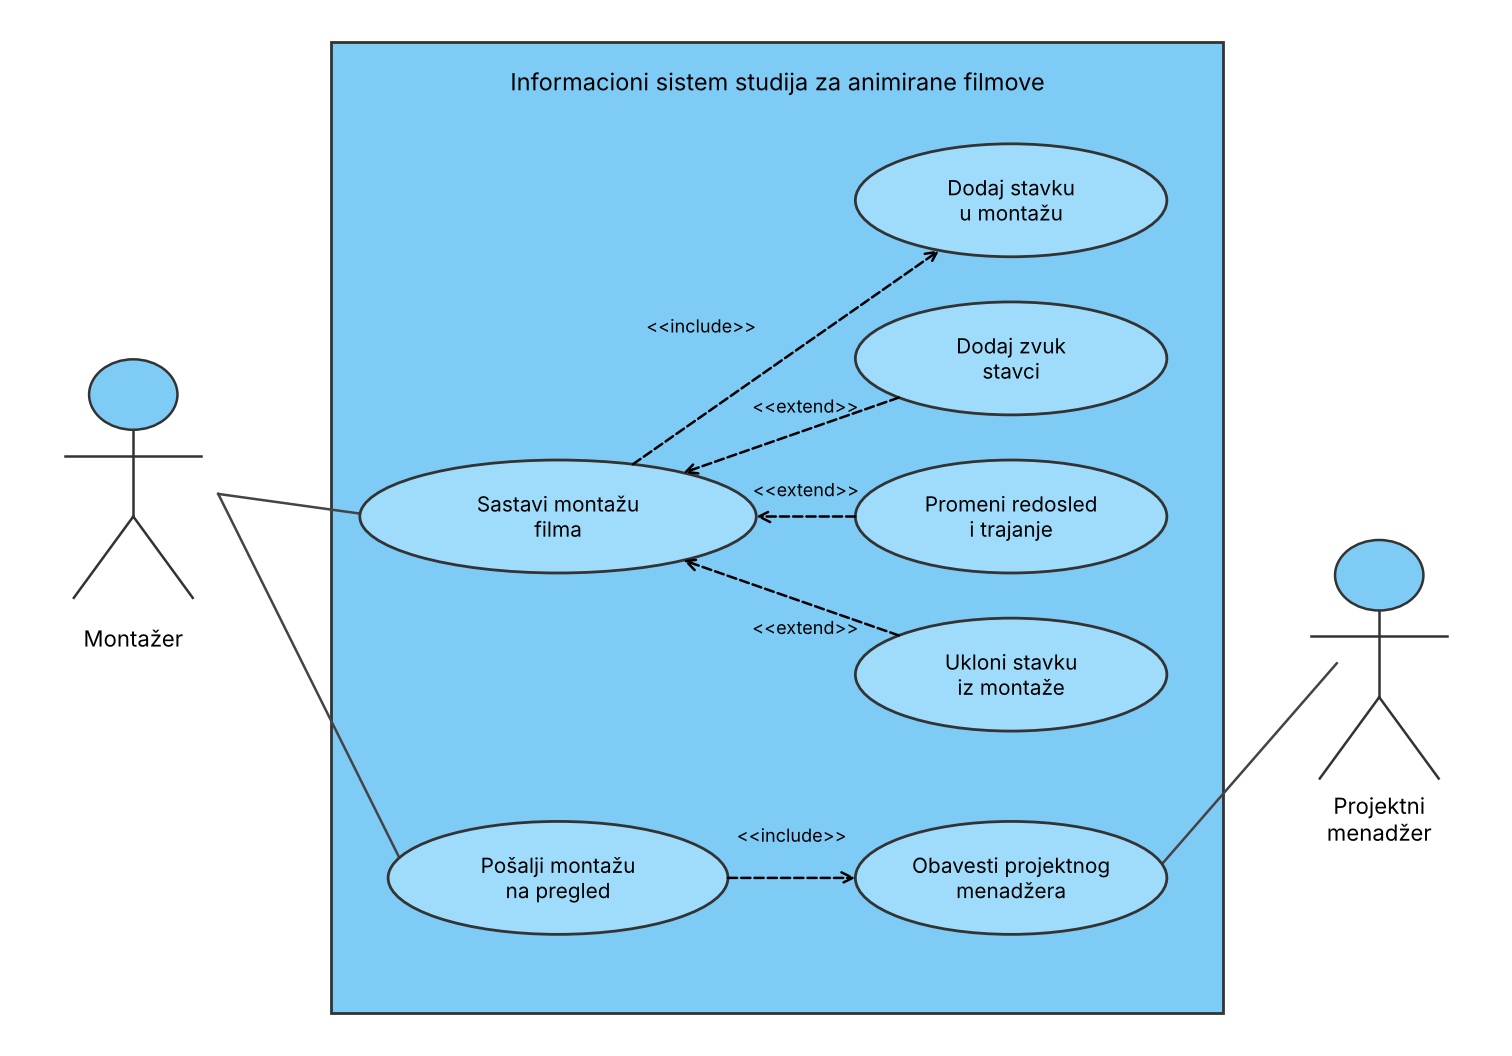
\includegraphics[width=\textwidth]{./dijagrami/dijagrami_slucajeva_upotrebe/montaza_filma.png}
	\caption{Dijagram slučaja upotrebe ,,Montaža filma''}
 \end{figure}

\begin{figure}[H]
	\centering
	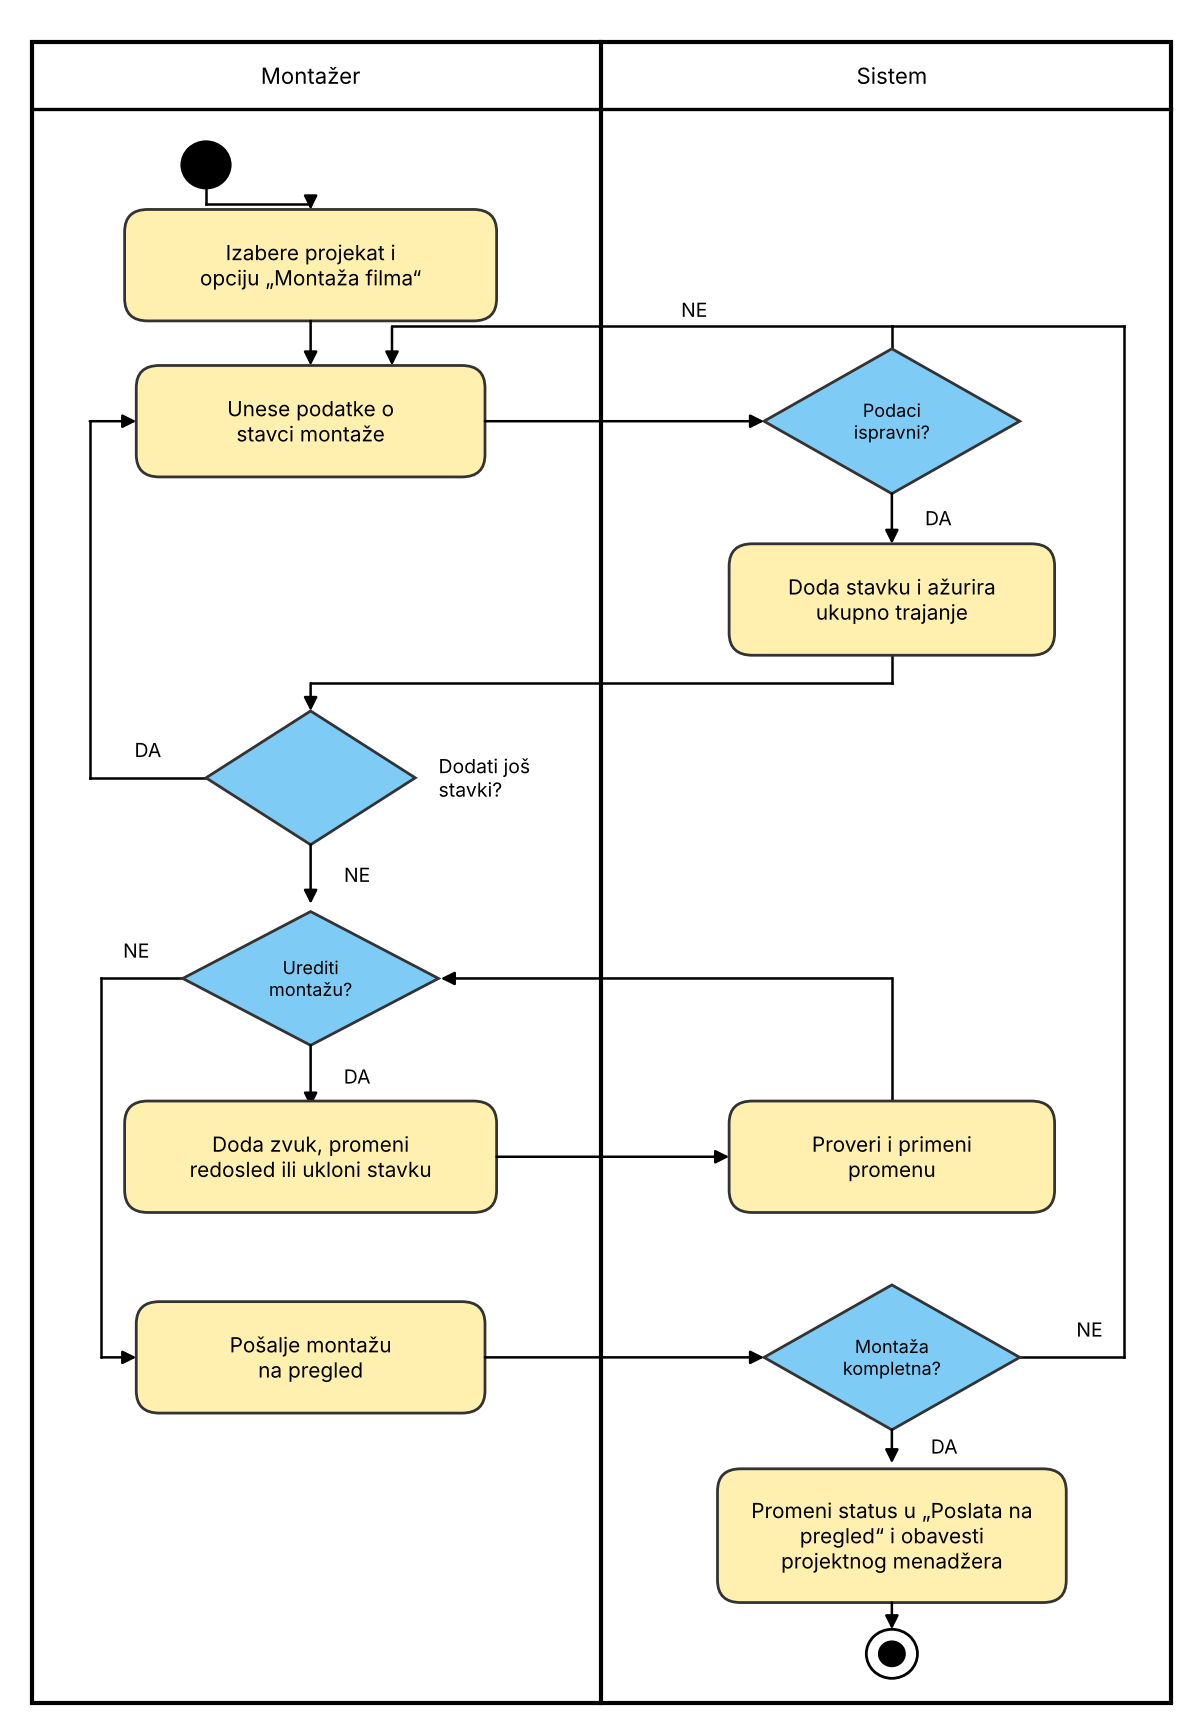
\includegraphics[width=\textwidth,height=0.8\textheight,keepaspectratio]{./dijagrami/dijagrami_aktivnosti/montaza_filma.png}
	\caption{Dijagram aktivnosti ,,Montaža filma''}
 \end{figure}

\begin{figure}[H]
	\centering
	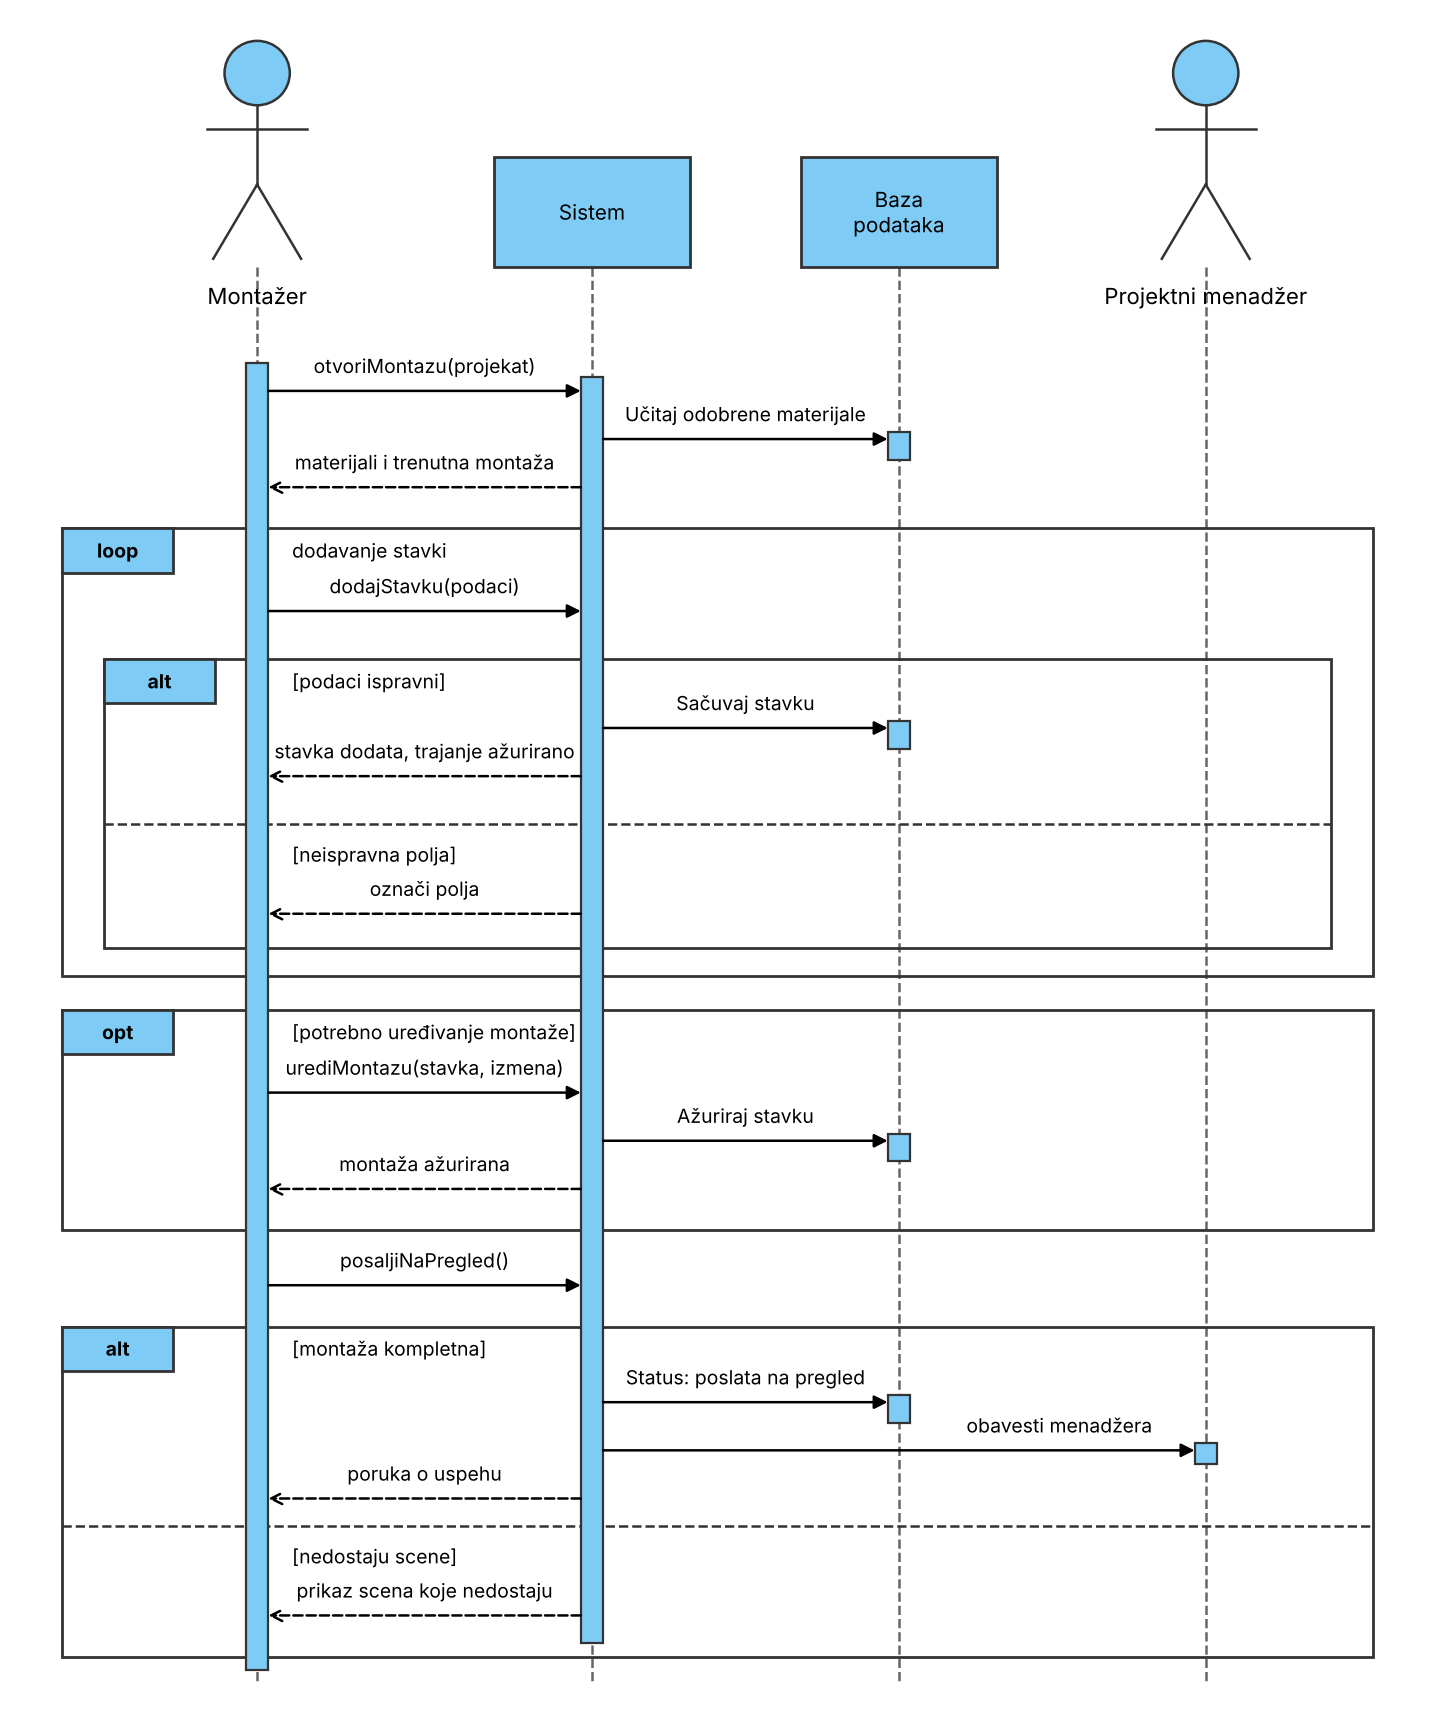
\includegraphics[width=\textwidth,height=0.8\textheight,keepaspectratio]{./dijagrami/dijagrami_sekvence/montaza_filma.png}
	\caption{Dijagram sekvence ,,Montaža filma''}
 \end{figure}

\newpage
